\documentclass[12pt]{article}
\usepackage[margin=1in]{geometry}

% PACKAGES
\usepackage{amsmath} % For extended formatting
%\usepackage{amssymb} % For math symbols
\usepackage{amsthm} % For proof environment
\usepackage{array} % For tables
\usepackage{enumerate} % For lists
\usepackage{extramarks} % For headers and footers
\usepackage{fancyhdr} % For custom headers
\usepackage{graphicx} % For inserting images
\usepackage{multicol} % For multiple columns
\usepackage{verbatim} % For displaying code
%\usepackage{tkz-euclide}
\usepackage{pgfplots}
\usepackage{tasks}

% SET UP HEADER AND FOOTER
\pagestyle{fancy}
\lhead{\MyCourse} % Top left header
\chead{\MyTopicTitle} % Top center header
\rhead{\MyAssignment} % Top right header
\lfoot{\MyCampus} % Bottom left footer
%\cfoot{June 14, 2022} % Bottom center footer
\rfoot{\MySemester} % Bottom right footer
\renewcommand\headrulewidth{0.4pt} % Size of the header rule
\renewcommand\footrulewidth{0.4pt} % Size of the footer rule
\setlength{\headheight}{14.49998pt}

\let\ds\displaystyle
\newcommand{\red}{\textcolor{red}}
\newcommand{\blue}{\textcolor{blue}}
\newcommand{\pink}{\textcolor{CarnationPink}}
\newcommand{\orange}{\textcolor{orange}}
\newcommand{\purple}{\textcolor{purple}}
\newcommand{\violet}{\textcolor{violet}}
\newcommand{\cyan}{\textcolor{cyan}}
\newcommand{\grn}{\textcolor{green}}
\newcommand{\uh}{\textcolor{ForestGreen}}

% ----------
% TITLES AND NAMES 
% ----------

\newcommand{\MyCourse}{Math 242}
\newcommand{\MyAssignment}{Worksheet 10}
\newcommand{\MySemester}{Fall 2024}
\newcommand{\MyCampus}{University of Hawaii at Manoa}


\pgfplotsset{compat=1.18} 
\begin{document}
\noindent Name: \hspace{4in}Section:
\vspace{0.5cm}



\begin{enumerate}
\item Test the series for convergence or divergence and name the test that you are using.
\begin{enumerate}
\item $\sum_{n=2}^{\infty}\frac{(n+1)(2n-2)^2}{(n-1)(n^2+3)^2}$
\vfill

\item $\sum_{n=1}^\infty (-1)^{n+1} n^{-2}\ln{n} $
\vfill
\item $\sum_{n=1}^\infty\left(1+\frac{1}{n}\right)^3e^{-n}$
\vfill
\item $\sum_{n=15}^{\infty} \frac{(\ln{n})^2}{n+14}$
\vfill



\newpage
\item $\sum_{n=0}^{\infty}\frac{(-3)^n}{(2n+1)!}$ (Use the ratio test)
\vfill
\item $\sum_{n=1}^{\infty}\left( \frac{-2n}{n+1}\right)^{5n}$

\vfill
\end{enumerate}
\item Test whether the series is absolutely convergent, conditionally convergent, or divergent.
\begin{enumerate}
\item $\sum_{n=1}^{\infty} \frac{n5^{2n}}{10^{n+1}}$
\vfill


\item $\sum_{n=2}^{\infty}\frac{(-1)^n}{n \ln{(n)}}$
\vfill
\end{enumerate}


 

\newpage
\item Approximate the sum of the series correct to four decimal places.\\
\[\sum_{n=1}^{\infty}\frac{(-1)^n}{n^6}\]
\vfill
\end{enumerate}
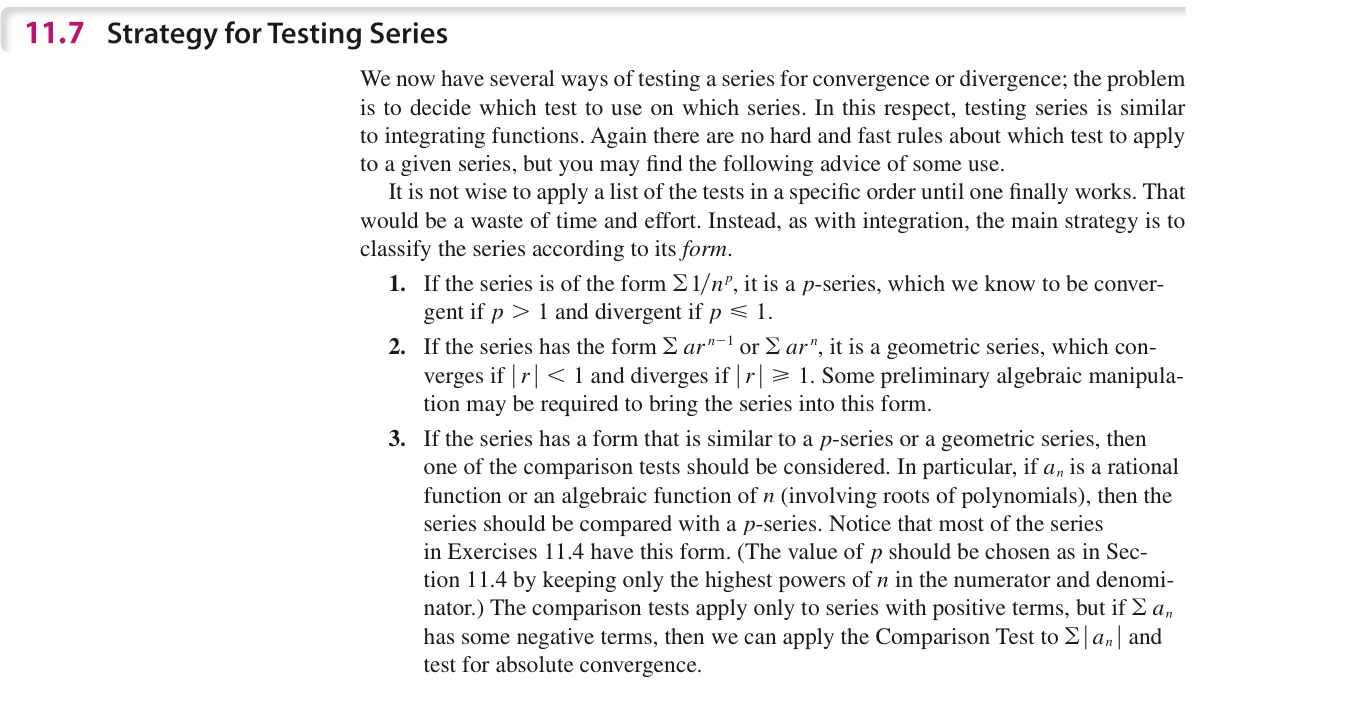
\includegraphics[width=19cm]{IMG_2703.jpg}
\newpage

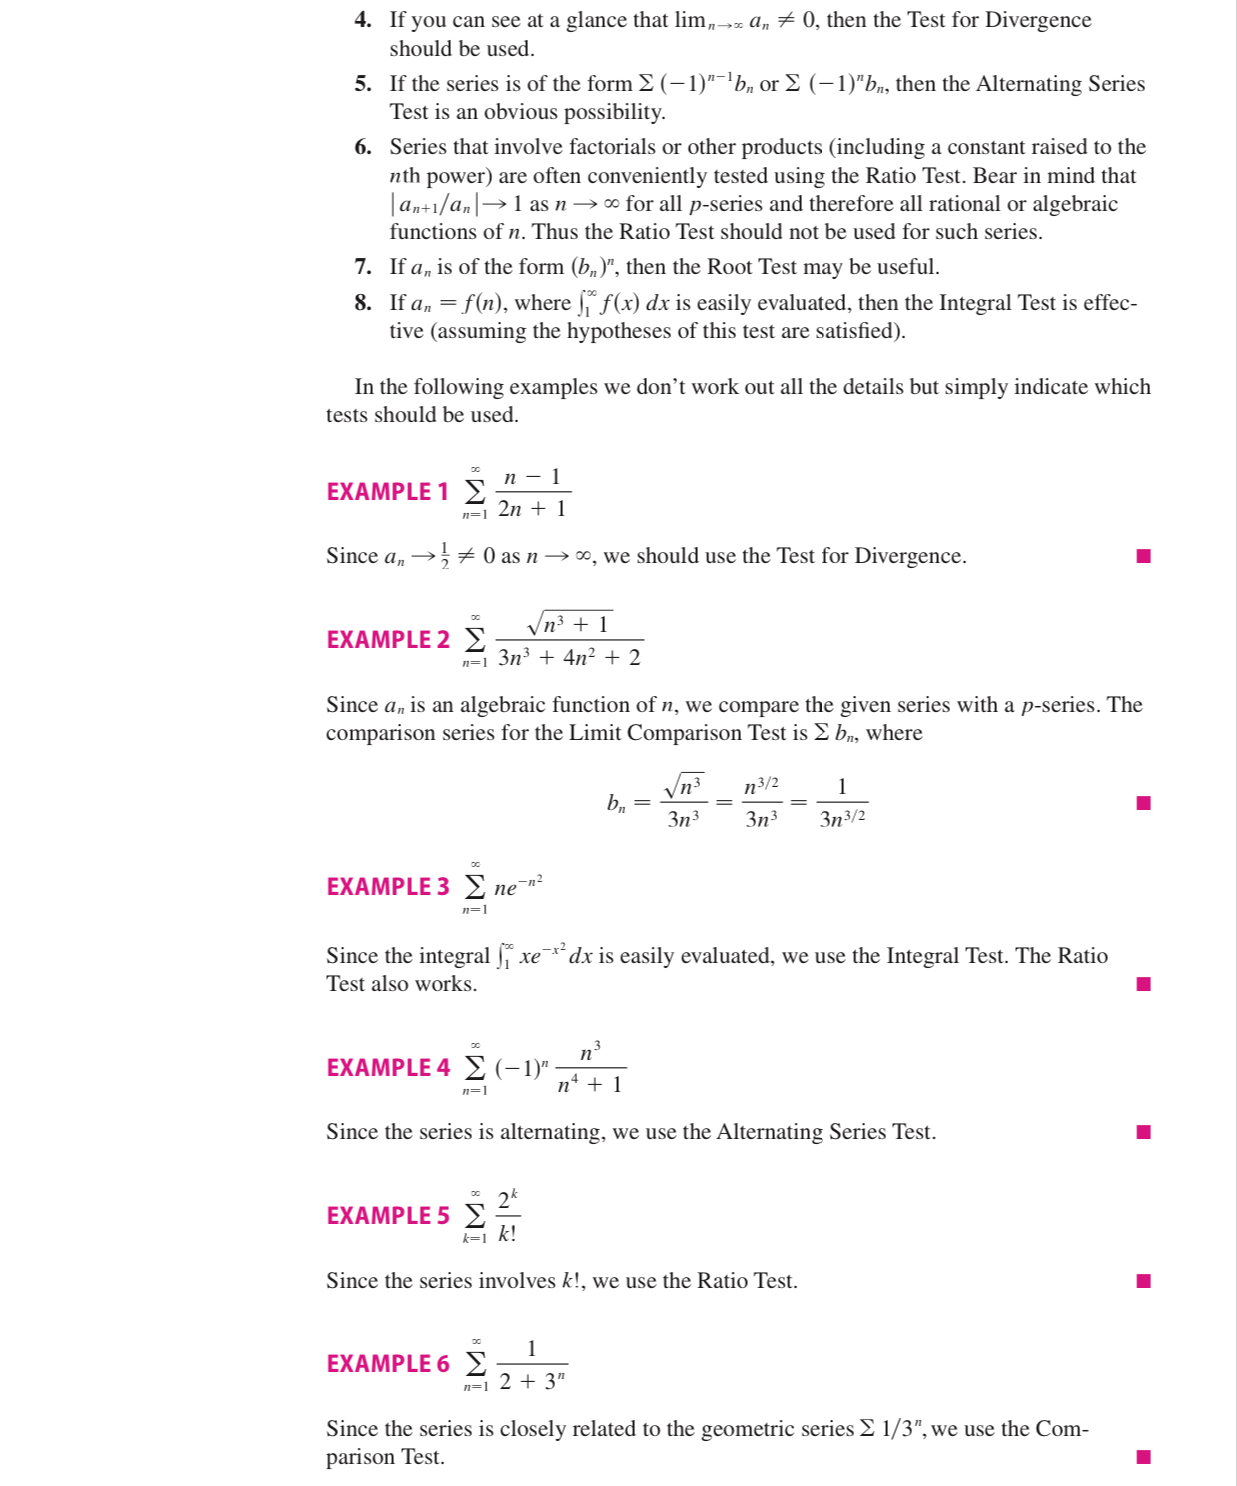
\includegraphics[width=18.5cm]{IMG_2702.jpg}

\end{document}